%%%%%%%%%%%%%%%%%%%%%%%%%%%%%%%%%%%%%%%%%
% Beamer Presentation
% LaTeX Template
% Version 2.0 (March 8, 2022)
%
% This template originates from:
% https://www.LaTeXTemplates.com
%
% Author:
% Vel (vel@latextemplates.com)
%
% License:
% CC BY-NC-SA 4.0 (https://creativecommons.org/licenses/by-nc-sa/4.0/)
%
%%%%%%%%%%%%%%%%%%%%%%%%%%%%%%%%%%%%%%%%%

%----------------------------------------------------------------------------------------
%	PACKAGES AND OTHER DOCUMENT CONFIGURATIONS
%----------------------------------------------------------------------------------------

\documentclass[
	11pt, % Set the default font size, options include: 8pt, 9pt, 10pt, 11pt, 12pt, 14pt, 17pt, 20pt
	%t, % Uncomment to vertically align all slide content to the top of the slide, rather than the default centered
	%aspectratio=169, % Uncomment to set the aspect ratio to a 16:9 ratio which matches the aspect ratio of 1080p and 4K screens and projectors
]{beamer}

\graphicspath{{Images/}{./}} % Specifies where to look for included images (trailing slash required)

\usepackage{booktabs} % Allows the use of \toprule, \midrule and \bottomrule for better rules in tables
\usepackage{palatino}
\usepackage[default]{opensans}

% For algorithm/pseudocode blocks (used in prior decks)
\usepackage{algorithm}
\usepackage[noend]{algpseudocode}

% For simple explanatory diagrams (consistent with prior decks)
\usepackage{tikz}
\usetikzlibrary{positioning,arrows.meta,calc}

%----------------------------------------------------------------------------------------
%	SELECT LAYOUT THEME
%----------------------------------------------------------------------------------------

% Beamer comes with a number of default layout themes which change the colors and layouts of slides. Below is a list of all themes available, uncomment each in turn to see what they look like.

%\usetheme{default}
%\usetheme{AnnArbor}
%\usetheme{Antibes}
%\usetheme{Bergen}
%\usetheme{Berkeley}
%\usetheme{Berlin}
%\usetheme{Boadilla}
\usetheme{CambridgeUS}
%\usetheme{Copenhagen}
%\usetheme{Darmstadt}
%\usetheme{Dresden}
%\usetheme{Frankfurt}
%\usetheme{Goettingen}
%\usetheme{Hannover}
%\usetheme{Ilmenau}
%\usetheme{JuanLesPins}
%\usetheme{Luebeck}
% \usetheme{Madrid}
%\usetheme{Malmoe}
%\usetheme{Marburg}
%\usetheme{Montpellier}
%\usetheme{PaloAlto}
%\usetheme{Pittsburgh}
%\usetheme{Rochester}
%\usetheme{Singapore}
%\usetheme{Szeged}
%\usetheme{Warsaw}

%----------------------------------------------------------------------------------------
%	SELECT COLOR THEME
%----------------------------------------------------------------------------------------

% Beamer comes with a number of color themes that can be applied to any layout theme to change its colors. Uncomment each of these in turn to see how they change the colors of your selected layout theme.

%\usecolortheme{albatross}
\usecolortheme{beaver}
%\usecolortheme{beetle}
%\usecolortheme{crane}
%\usecolortheme{dolphin}
%\usecolortheme{dove}
%\usecolortheme{fly}
%\usecolortheme{lily}
%\usecolortheme{monarca}
%\usecolortheme{seagull}
%\usecolortheme{seahorse}
%\usecolortheme{spruce}
%\usecolortheme{whale}
%\usecolortheme{wolverine}

%----------------------------------------------------------------------------------------
%	SELECT FONT THEME & FONTS
%----------------------------------------------------------------------------------------

% Beamer comes with several font themes to easily change the fonts used in various parts of the presentation. Review the comments beside each one to decide if you would like to use it. Note that additional options can be specified for several of these font themes, consult the beamer documentation for more information.

\usefonttheme{default} % Typeset using the default sans serif font
%\usefonttheme{serif} % Typeset using the default serif font (make sure a sans font isn't being set as the default font if you use this option!)
%\usefonttheme{structurebold} % Typeset important structure text (titles, headlines, footlines, sidebar, etc) in bold
%\usefonttheme{structureitalicserif} % Typeset important structure text (titles, headlines, footlines, sidebar, etc) in italic serif
%\usefonttheme{structuresmallcapsserif} % Typeset important structure text (titles, headlines, footlines, sidebar, etc) in small caps serif

%------------------------------------------------

%\usepackage{mathptmx} % Use the Times font for serif text
\usepackage{palatino} % Use the Palatino font for serif text

%\usepackage{helvet} % Use the Helvetica font for sans serif text
\usepackage[default]{opensans} % Use the Open Sans font for sans serif text
%\usepackage[default]{FiraSans} % Use the Fira Sans font for sans serif text
%\usepackage[default]{lato} % Use the Lato font for sans serif text

%----------------------------------------------------------------------------------------
%	SELECT INNER THEME
%----------------------------------------------------------------------------------------

% Inner themes change the styling of internal slide elements, for example: bullet points, blocks, bibliography entries, title pages, theorems, etc. Uncomment each theme in turn to see what changes it makes to your presentation.

%\useinnertheme{default}
\useinnertheme{circles}
%\useinnertheme{rectangles}
%\useinnertheme{rounded}
%\useinnertheme{inmargin}

%----------------------------------------------------------------------------------------
%	SELECT OUTER THEME
%----------------------------------------------------------------------------------------

% Outer themes change the overall layout of slides, such as: header and footer lines, sidebars and slide titles. Uncomment each theme in turn to see what changes it makes to your presentation.

%\useoutertheme{default}
%\useoutertheme{infolines}
%\useoutertheme{miniframes}
%\useoutertheme{smoothbars}
%\useoutertheme{sidebar}
%\useoutertheme{split}
%\useoutertheme{shadow}
%\useoutertheme{tree}
%\useoutertheme{smoothtree}

%\setbeamertemplate{footline} % Uncomment this line to remove the footer line in all slides
%\setbeamertemplate{footline}[page number] % Uncomment this line to replace the footer line in all slides with a simple slide count

%\setbeamertemplate{navigation symbols}{} % Uncomment this line to remove the navigation symbols from the bottom of all slides

%----------------------------------------------------------------------------------------
%	PRESENTATION INFORMATION
%----------------------------------------------------------------------------------------

% The short title in the optional parameter appears at the bottom of every slide, the full title in the main parameter is only on the title page
\title[\textsc{NS-BRKGA} for MOPCI]{A Non-dominated Sorting Biased Random-Key Genetic Algorithm for the Multi-Objective Physical Cell Identity Assignment Problem}

% \subtitle{Optional Subtitle} % Presentation subtitle, remove this command if a subtitle isn't required

% Presenter name(s), the optional parameter can contain a shortened version to appear on the bottom of every slide, while the main parameter will appear on the title slide
\author[L. H. P. M. et al.]{
Luis H. P. Mendes \and
F\'{a}bio L. Usberti \and
M\'{a}rio C. San Felice \and
Carlos E. de Andrade
}

% Your institution, the optional parameter can be used for the institution shorthand and will appear on the bottom of every slide after author names, while the required parameter is used on the title slide and can include your email address or additional information on separate lines
\institute[UNICAMP / UFSCar / AT\&T]{
Institute of Computing -- University of Campinas (UNICAMP)\\
Department of Computing -- Federal University of S\~{a}o Carlos (UFSCar)\\
AT\&T Labs Research\\
\smallskip
\texttt{luis.mendes@ic.unicamp.br}
}

% Presentation date or conference/meeting name, the optional parameter can contain a shortened version to appear on the bottom of every slide, while the required parameter value is output to the title slide
\date[MIC 2026]{16th Metaheuristics International Conference (MIC 2026)}

\newcommand{\NIGDplus}{\mathit{NIGD^{+}}}
\newcommand{\HVR}{\mathit{HVR}}

%----------------------------------------------------------------------------------------

\begin{document}

%----------------------------------------------------------------------------------------
%	TITLE SLIDE
%----------------------------------------------------------------------------------------

\begin{frame}
\titlepage % Output the title slide, automatically created using the text entered in the PRESENTATION INFORMATION block above
\end{frame}

%----------------------------------------------------------------------------------------
%	TABLE OF CONTENTS SLIDE
%----------------------------------------------------------------------------------------

% The table of contents outputs the sections and subsections that appear in your presentation, specified with the standard \section and \subsection commands. You may either display all sections and subsections on one slide with \tableofcontents, or display each section at a time on subsequent slides with \tableofcontents[pausesections]. The latter is useful if you want to step through each section and mention what you will discuss.

\begin{frame}
\frametitle{Presentation Overview} % Slide title, remove this command for no title
	
\tableofcontents % Output the table of contents (all sections on one slide)
%\tableofcontents[pausesections] % Output the table of contents (break sections up across separate slides)
\end{frame}

%----------------------------------------------------------------------------------------
%	PRESENTATION BODY SLIDES
%----------------------------------------------------------------------------------------

% Sections are added in order to organize your presentation into discrete blocks, all sections and subsections are automatically output to the table of contents as an overview of the talk but NOT output in the presentation as separate slides

%========================================================================================
\section{Motivation and context}

\begin{frame}[plain]
\begin{center}
{\Huge Motivation\\and context}
\end{center}
\end{frame}

%----------------------------------------------------------------------------------------

\begin{frame}
\frametitle{Why PCI assignment is a hard (and practical) optimization task}

\begin{itemize}
\item Each LTE/5G cell must broadcast a \textbf{Physical Cell Identity (PCI)} so UEs can detect and distinguish cells.

\item The PCI space is \textbf{limited} (e.g., $\mathbf{504}$ values in LTE; $\mathbf{1008}$ in 5G), so PCIs must be \textbf{reused}.

\item Poor reuse leads to technological conflicts (collisions, confusions, modulo-$k$ interference) that degrade measurements and mobility.

\item Operators also care about \textbf{operational objectives}: minimize disruptive PCI changes and avoid deployment failures during staged rollouts.
\end{itemize}

% Speaker framing: “This is not only about feasibility; it is about managing trade-offs between interference, deployment safety, and stability.”
\end{frame}

%----------------------------------------------------------------------------------------
\begin{frame}
\frametitle{The conflicts we must avoid (intuition)}

\begin{columns}[T,onlytextwidth]
\column{0.58\textwidth}
\begin{itemize}
\item \textbf{Collision}: adjacent cells share the same PCI $\rightarrow$ UE cannot distinguish signals.

\item \textbf{Top-neighbor modulo-$\mathbf{k}$ collision}: critical neighbors have PCIs congruent modulo $k$ $\rightarrow$ reference signals interfere.

\item \textbf{Confusion}: a cell has \emph{two} distinct neighbors with the same PCI $\rightarrow$ ambiguous handover target.

\item \textbf{PCI shuffle (during rollout)}: a cell is assigned a new PCI equal to a neighbor's \emph{current} PCI $\rightarrow$ transient collision/confusion and deployment failure.
\end{itemize}

\column{0.42\textwidth}
\centering
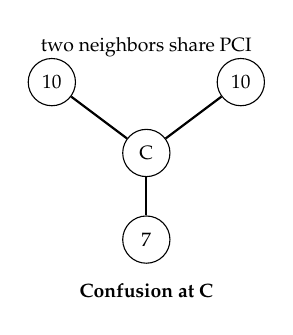
\begin{tikzpicture}[
node/.style={circle,draw,minimum size=6mm,inner sep=0pt},
edge/.style={-Latex,thick},
scale=1.0
]
\node[node] (c) at (0,0) {\scriptsize C};
\node[node] (a) at (-1.2,0.9) {\scriptsize 10};
\node[node] (b) at (1.2,0.9) {\scriptsize 10};
\node[node] (d) at (0,-1.1) {\scriptsize 7};

\draw[thick] (c) -- (a);
\draw[thick] (c) -- (b);
\draw[thick] (c) -- (d);

\node at (0,1.35) {\scriptsize two neighbors share PCI};

\node[align=center] at (0,-1.75) {\scriptsize \textbf{Confusion at C}};
\end{tikzpicture}

\vspace{0.2em}

{\scriptsize (schematic)}
\end{columns}

% Speaker note: Use this slide to calibrate terminology (collision vs confusion vs modulo-$k$ vs shuffle).
\end{frame}

%----------------------------------------------------------------------------------------
\begin{frame}
\frametitle{Main contributions}

\begin{enumerate}
\item We propose a \textbf{Non-dominated Sorting \textsc{BRKGA} (\textsc{NS-BRKGA})} to solve the \textbf{multi-objective} PCI assignment problem with conflicting objectives.

\item We design a \textbf{random-key encoding + specialized decoder} that combines:
\begin{itemize}
\item fast best-effort \textbf{constraint repair},
\item \textbf{lexicographically guided} local search, and
\item \textbf{genotype feedback} (re-encoding improvements into chromosomes).
\end{itemize}

\item We benchmark on \textbf{291 real-world instances} against five representative MOEAs (incl. \textsc{NSGA-II}), showing \textbf{stronger Pareto fronts} under the same time budget.
\end{enumerate}

% Speaker note: Be explicit about novelty: the memetic decoder + feedback is what makes the framework effective on highly constrained instances.
\end{frame}

%========================================================================================
\section{Problem definition}

\begin{frame}[plain]
\begin{center}
{\Huge Problem\\definition}
\end{center}
\end{frame}

%----------------------------------------------------------------------------------------
\begin{frame}
\frametitle{Modeling the network and neighborhoods}

We model the network as an undirected graph $G = (V, E)$:
\begin{itemize}
\item $V$: cells; \qquad $E$: neighbor/interference relations.
\end{itemize}

The edge set is partitioned:
\[
E = T \cup N,\qquad T \cap N = \emptyset,
\]
\begin{itemize}
\item $T$: \textbf{top-neighbors} (critical relations) where modulo-$k$ collisions are \emph{forbidden};
\item $N$: regular neighbors where direct collisions are forbidden, and modulo-$k$ collisions are undesirable.
\end{itemize}

Second-level neighbors (used to model confusions):
\[
S = \{(u, w) \mid (u, v) \in E,\ (v, w) \in E,\ (u, w) \notin E\}.
\]

% Speaker note: This slide sets notation you'll reuse on the constraints/objectives slides. Keep it tight.
\end{frame}

%----------------------------------------------------------------------------------------
\begin{frame}
\frametitle{Decision variables and hard constraints}

Decision variable: assign each cell $v \in V$ an integer PCI $x_{v} \in AP \subseteq \{0, 1, \dots,PCI_{\max}\}$.

\bigskip

\textbf{Hard constraints (must hold):}
\begin{enumerate}
\item \textbf{Collision-freeness} (no adjacent equal PCIs):
\[
x_{u} \neq x_{v},\quad \forall (u, v) \in E.
\]

\item \textbf{Top-neighbor modulo-$\mathbf{k}$ collision-freeness}:
\[
x_{u} \not\equiv x_{v} \ (\mathrm{mod}\ k),\quad \forall (u, v) \in T.
\]

\item \textbf{Confusion-freeness} (no two second-level neighbors share a PCI):
\[
x_{u} \neq x_{v}, \quad \forall (u, v) \in S.
\]
\end{enumerate}

% Speaker framing: “We treat these as inviolable—everything else is optimized as a trade-off.”
\end{frame}

%----------------------------------------------------------------------------------------
\begin{frame}
\frametitle{Three objectives (trade-offs)}

Let $\mathbb{I}(\cdot)$ be the indicator function and $O_{v}$ the original PCI of cell $v$.

\begin{enumerate}
\item \textbf{Modulo-$\mathbf{k}$ collisions on regular neighbors} (interference):
\[
f_{1}(x) = \sum_{(u, v) \in N}{\mathbb{I}\big(x_{u} \equiv x_{v} \ (\mathrm{mod}\ k)\big)}.
\]

\item \textbf{PCI shuffles} (deployment safety during batched rollouts):
\[
f_{2}(x) = \sum_{(u, v) \in E \cup S}{\Big(\mathbb{I}(x_{u} = O_{v}) + \mathbb{I}(x_{v} = O_{u})\Big)}.
\]

\item \textbf{Total PCI changes} (stability / renumbering cost):
\[
f_{3}(x) = \sum_{v \in V}{\mathbb{I}(x_{v} \neq O_{v})}.
\]
\end{enumerate}

\medskip
Goal: approximate the \textbf{Pareto front} for $(f_{1}, f_{2}, f_{3})$ over feasible assignments.

% Speaker note: Emphasize that this is a constrained MOP, not just a graph coloring problem.
\end{frame}

%========================================================================================
\section{Proposed method}

\begin{frame}[plain]
\begin{center}
{\Huge Proposed method\\(\textsc{NS-BRKGA})}
\end{center}
\end{frame}

%----------------------------------------------------------------------------------------
\begin{frame}
\frametitle{\textsc{NS-BRKGA} at a glance: random keys + memetic decoder}

\begin{center}
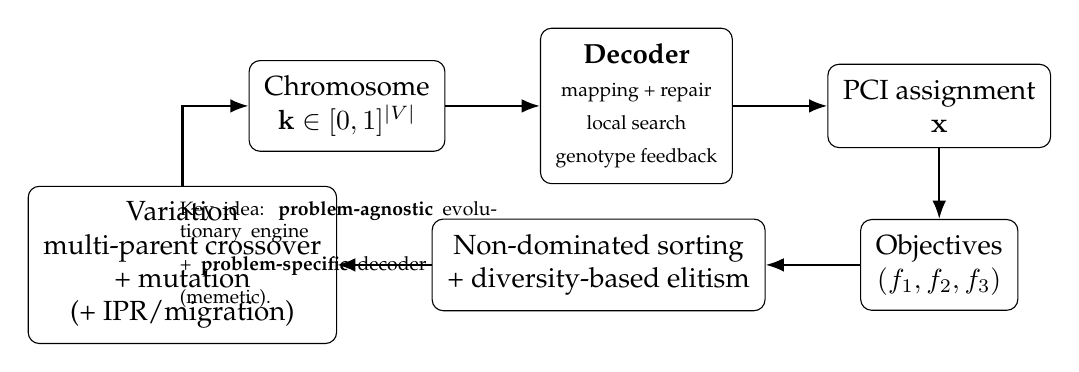
\begin{tikzpicture}[
box/.style={draw, rounded corners, align=center, inner sep=0.55em},
arr/.style={-Latex, thick},
node distance=1.0cm
]
\node[box] (rk) {Chromosome\\$\mathbf{k} \in [0, 1]^{|V|}$};

\node[box, right=1.2cm of rk] (dec) {\textbf{Decoder}\\
\scriptsize mapping + repair\\
\scriptsize local search\\
\scriptsize genotype feedback};

\node[box, right=1.2cm of dec] (x) {PCI assignment\\$\mathbf{x}$};

\node[box, below=0.9cm of x] (obj) {Objectives\\$(f_{1}, f_{2}, f_{3})$};

\node[box, left=1.2cm of obj] (sel) {Non-dominated sorting\\+ diversity-based elitism};

\node[box, left=1.2cm of sel] (var) {Variation\\multi-parent crossover\\+ mutation\\(+ IPR/migration)};

\draw[arr] (rk) -- (dec);
\draw[arr] (dec) -- (x);
\draw[arr] (x) -- (obj);
\draw[arr] (obj) -- (sel);
\draw[arr] (sel) -- (var);
\draw[arr] (var) |- (rk);

\node[align=left, below=0.5cm of rk, text width=0.35\textwidth] {\scriptsize
Key idea: \textbf{problem-agnostic} evolutionary engine\\
+\ \textbf{problem-specific} decoder (memetic).
};
\end{tikzpicture}
\end{center}

% Speaker framing: “The evolutionary operators stay in the continuous space; all discrete complexity is pushed into the decoder.”
\end{frame}

%----------------------------------------------------------------------------------------
\begin{frame}
\frametitle{Solution representation}

A chromosome is a vector of random keys:
\[
\mathbf{k} = (k_{v})_{v \in V}, \qquad k_{v} \sim \mathcal{U}[0, 1].
\]

Let $AP$ be the sorted list of allowed PCIs, with $m = |AP|$.

\bigskip

\textbf{Deterministic decoding (initial assignment):}
\[
x_{v} \;=\; AP\!\left[\left\lfloor k_v\cdot m \right\rfloor\right].
\]

\begin{itemize}
\item This decoding is fast, but it can yield \textbf{infeasible} assignments.
\item Feasibility is enforced by an embedded repair + local improvement phase.
\end{itemize}

% Speaker note: Emphasize “continuous search, discrete feasibility”.
\end{frame}

%----------------------------------------------------------------------------------------
\begin{frame}
\frametitle{Decoder step 1: quantify and repair hard-constraint violations}

Violation counts used by the decoder:
\[
\begin{aligned}
v_{\mathrm{col}}(\mathbf{x})  &= \sum_{(u, v) \in E}\mathbb{I}(x_{u} = x_{v}),\\
v_{\mathrm{tn}}(\mathbf{x})   &= \sum_{(u, v) \in T}\mathbb{I}\big(x_{u} \equiv x_{v}\ (\mathrm{mod}\ k)\big),\\
v_{\mathrm{conf}}(\mathbf{x}) &= \sum_{(u, v) \in S}\mathbb{I}(x_{u} = x_{v}).
\end{aligned}
\]
A solution is feasible iff $v_{\mathrm{col}} = v_{\mathrm{tn}} = v_{\mathrm{conf}} = 0$.

\medskip
\textbf{Greedy best-effort repair (high level):}
\begin{enumerate}
\item Find cells involved in violations: $U \subseteq V$.
\item Pick $v \in U$ with the most incident violations (tie: higher degree).
\item Try each $p \in AP$: set $x_{v} \leftarrow p$ and choose the move with smallest $v_{\mathrm{col}} + v_{\mathrm{tn}} + v_{\mathrm{conf}}$.
\item Repeat until no move improves the total violation count.
\end{enumerate}

% Speaker note: This is where feasibility becomes “cheap”, enabling robustness on squz instances.
\end{frame}

%----------------------------------------------------------------------------------------
\begin{frame}
\frametitle{Decoder step 1: quantify and repair hard-constraint violations}

Violation counts used by the decoder:
\[
\begin{aligned}
v_{\mathrm{col}}(\mathbf{x}) &= \sum_{(u, v) \in E}\mathbb{I}(x_{u} = x_{v}),\\
v_{\mathrm{tn}}(\mathbf{x})  &= \sum_{(u, v) \in T}\mathbb{I}\big(x_{u} \equiv x_{v}\ (\mathrm{mod}\ k)\big),\\
v_{\mathrm{conf}}(\mathbf{x})&= \sum_{(u, v) \in S}\mathbb{I}(x_{u} = x_{v}).
\end{aligned}
\]
A solution is feasible iff $v_{\mathrm{col}} = v_{\mathrm{tn}} = v_{\mathrm{conf}} = 0$.

\medskip
\textbf{Greedy best-effort repair (high level):}
\begin{enumerate}
\item Find cells involved in violations: $U \subseteq V$.
\item Pick $v \in U$ with the most incident violations (tie: higher degree).
\item Try each $p \in AP$: set $x_{v} \leftarrow p$ and choose the move with smallest $v_{\mathrm{col}} + v_{\mathrm{tn}} + v_{\mathrm{conf}}$.
\item Repeat until no move improves the total violation count.
\end{enumerate}

% Speaker note: This is where feasibility becomes “cheap”, enabling robustness on squz instances.
\end{frame}

%----------------------------------------------------------------------------------------
\begin{frame}
\frametitle{Decoder step 1b: penalize residual infeasibility (so elites remain feasible)}

If repair cannot remove all violations, we penalize the first objective:
\[
\tilde{f_{1}}(\mathbf{x}) = f_{1}(\mathbf{x}) + M\cdot\big(v_{\mathrm{col}}(\mathbf{x}) + v_{\mathrm{tn}}(\mathbf{x}) + v_{\mathrm{conf}}(\mathbf{x})\big),
\]
with a large constant $M$ (set as $M = |N| + 1$ in the paper).

\bigskip

Returned fitness is:
\[
\big(\tilde{f_{1}}(\mathbf{x}),\ f_{2}(\mathbf{x}),\ f_{3}(\mathbf{x})\big).
\]

\begin{itemize}
\item Any remaining hard-constraint violation makes $\tilde{f_{1}}$ worse than the worst feasible $f_{1}$ value.
\item This prevents infeasible solutions from dominating feasible ones.
\end{itemize}

% Speaker note: The “penalize only f1” design is nontrivial—explain quickly why it works.
\end{frame}

%----------------------------------------------------------------------------------------
\begin{frame}
\frametitle{Decoder step 2: lexicographically guided local search}

Once feasible, we run local search over \textbf{feasible single-cell moves}:
\[
x_{v} \leftarrow p, \quad p \in AP \setminus \{x_{v}\}\ \text{and move preserves feasibility.}
\]

\textbf{Move acceptance (inside the decoder):} first-improvement under a lexicographic order
\[
(a_{1}, a_{2}, a_{3}) \prec (b_{1}, b_{2}, b_{3})\ \Leftrightarrow\ 
\begin{cases}
a_{1} < b_{1},\ \text{or}\\
a_{1} = b_{1}\ \wedge\ a_{2} < b_{2},\ \text{or}\\
a_{1} = b_{1}\ \wedge\ a_{2} = b_{2}\ \wedge\ a_{3} < b_{3}.
\end{cases}
\]

\begin{itemize}
\item Local search prioritizes operational objectives in the order $(f_{1}, f_{2}, f_{3})$.
\item Example (from the paper): increasing $f_{3}$ is accepted only if it improves $f_{2}$ or $f_{1}$.
\end{itemize}

% Speaker note: Clarify: global selection is Pareto-based; lexicographic is only an intensification/tie-breaker inside the decoder.
\end{frame}

%----------------------------------------------------------------------------------------
\begin{frame}
\frametitle{Decoder step 3: genotype feedback (inherit local-search improvements)}

After local search improves $\mathbf{x}$, we \textbf{re-encode} the solution back into the chromosome.

\medskip
If $x_{v} = AP[j]$ for $j \in \{0, \dots, |AP| - 1\}$, set:
\[
k_{v} \leftarrow \frac{j + 0.5}{|AP|}\quad\Rightarrow\quad \left\lfloor k_{v} \cdot |AP|\right\rfloor = j.
\]

\begin{itemize}
\item The decoder becomes a \textbf{memetic operator}: improvements are not lost.
\item Evolutionary operators can now recombine and propagate locally improved building blocks.
\end{itemize}

% Speaker note: This is the key “BRKGA-friendly” way to do local search.
\end{frame}

%----------------------------------------------------------------------------------------
\begin{frame}
\frametitle{Evolutionary engine: \textsc{NSGA}-style ranking + \textsc{BRKGA} variation + intensification}

\begin{itemize}
\item \textbf{Population ranking:} Pareto dominance via non-dominated sorting.
\item \textbf{Elitism:} prioritize non-dominated solutions, then maximize \textbf{genotypic diversity} (distance in random-key space).
\item \textbf{Variation:} biased \textbf{multi-parent crossover} ($\pi > 2$) + \textbf{polynomial mutation}.
\end{itemize}

\bigskip

\textbf{Explicit intensification/diversification (paper configuration):}
\begin{itemize}
\item Implicit Path-Relinking (IPR) every $500$ generations.
\item Multi-population scheme ($p = 3$) with migration every 200 generations ($k = 30$ elites migrated).
\item Stagnation handling:
\begin{itemize}
\item \emph{shaking} after $200$ stagnant generations,
\item partial \emph{reset} after $500$ stagnant generations.
\end{itemize}
\end{itemize}

% Speaker note: Put the emphasis on “why”: robustness + scalability (decoder does heavy lifting; engine prevents premature convergence).
\end{frame}

%----------------------------------------------------------------------------------------
\begin{frame}
\frametitle{Parameter settings used in the experiments (reference)}

\begin{table}[!htbp]
\centering
\resizebox{\textwidth}{!}{
\begin{tabular}{ll}
\toprule
\textbf{Parameter}                              & \textbf{Value}                                                    \\
\midrule
Population size $|P|$ (per subpopulation)       & $300$                                                             \\
Parent count $\pi$ (elitist $\pi_e$)            & $3$ (with $\pi_e = 2$ elites)                                     \\
Elite fraction $p^{e}_{\min}$ -- $p^{e}_{\max}$ & $0.10$ -- $0.30$                                                  \\
Bias function $\Phi(r)$                         & $1/\sqrt{r}$                                                      \\
Mutation probability $p_{m}$ (index $\eta_{m}$) & $0.01$ ($\eta_{m} = 50$)                                          \\
Number of subpopulations $p$                    & $3$                                                               \\
Migration interval (gen), size $k$              & $200$ gen, $k = 30$ solutions                                     \\
IPR interval (gen)                              & $500$ gen                                                         \\
Shaking trigger (stagnant gen)                  & $200$ gen ($p_{\text{shake}} = 0.33$, $\eta_{\text{shake}} = 20$) \\
Reset trigger (stagnant gen)                    & $500$ gen ($p_{\text{reset}} = 0.20$)                             \\
\bottomrule
\end{tabular}
}
\label{tab:nsbrkga_params}
\end{table}

% Speaker note: Optional slide. If time is tight, skip. Use it only if asked about parameters.
\end{frame}

%========================================================================================
\section{Experimental setup}

\begin{frame}[plain]
\begin{center}
{\Huge Experimental\\setup}
\end{center}
\end{frame}

%----------------------------------------------------------------------------------------
\begin{frame}
\frametitle{Benchmark instances and protocol}

\begin{itemize}
\item \textbf{Benchmark:} $291$ real-world MOPCI instances introduced by prior work, sizes from $\mathbf{30}$ up to $\mathbf{4125}$ cells.

\item \textbf{Instance types (PCI groups):}
\begin{itemize}
\item \texttt{full}: $AP = \{0, \dots, 1007\}$ (least constrained),
\item \texttt{orig}: $AP = \{\min(O), \dots, \max(O)\}$,
\item \texttt{squz}: minimal contiguous $AP$ still admitting a feasible solution (most constrained).
\end{itemize}

\item \textbf{Budget:} $15$ minutes per run, $5$ independent runs per instance.
\item Each run returns a non-dominated archive (capped for reporting).
\end{itemize}

% Speaker note: Define “squz” clearly: this is where feasibility is hardest and where the decoder matters most.
\end{frame}


%----------------------------------------------------------------------------------------
\begin{frame}
\frametitle{Baselines and performance indicators}

\textbf{Baselines (same time budget):}
\begin{itemize}
\item \textsc{NSGA-II}, \textsc{MOEA/D-DE}, \textsc{NSPSO}, \textsc{MHACO}, \textsc{IHS}.
\end{itemize}

\bigskip

\textbf{Indicators (computed per instance):}
\begin{itemize}
\item $\mathbf{\NIGDplus}$ (lower is better): convergence to a reference front.
\item $\mathbf{\HVR}$ (higher is better): dominated hypervolume ratio vs reference front.
\end{itemize}

\bigskip

\textbf{Reference front:} pooled non-dominated set across all algorithms and runs (filtered for size).

% Speaker note: You can skip indicator details unless asked; the key is: two complementary metrics, same runtime budget.
\end{frame}

%========================================================================================
\section{Main computational results}

\begin{frame}[plain]
\begin{center}
{\Huge Main\\computational results}
\end{center}
\end{frame}

%----------------------------------------------------------------------------------------
\begin{frame}
\frametitle{Overall performance across all $291$ instances}

\begin{figure}
\centering
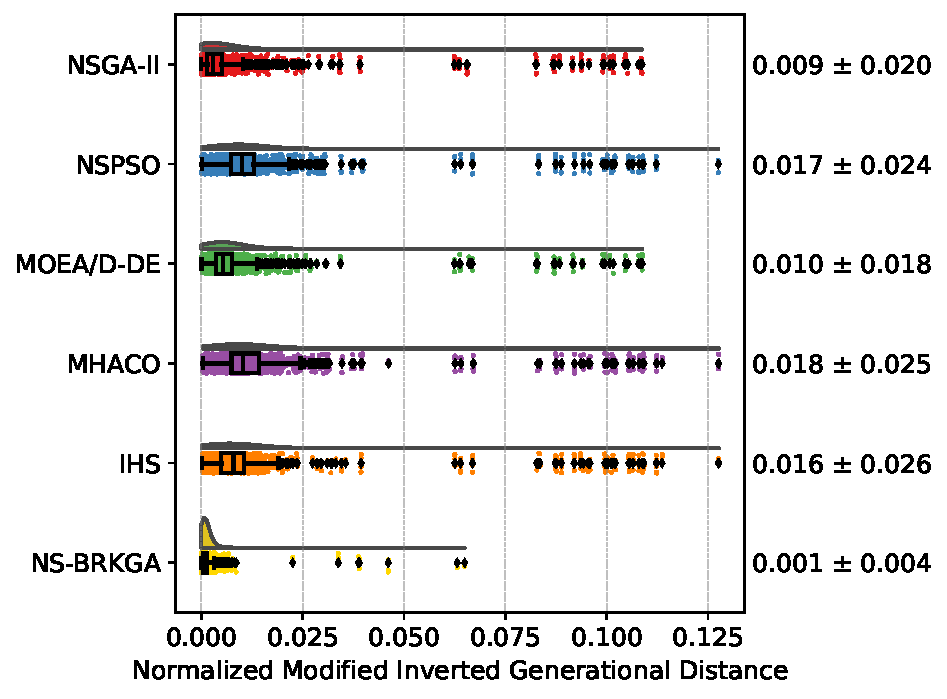
\includegraphics[width=0.48\textwidth]{figs/igd_plus.pdf}
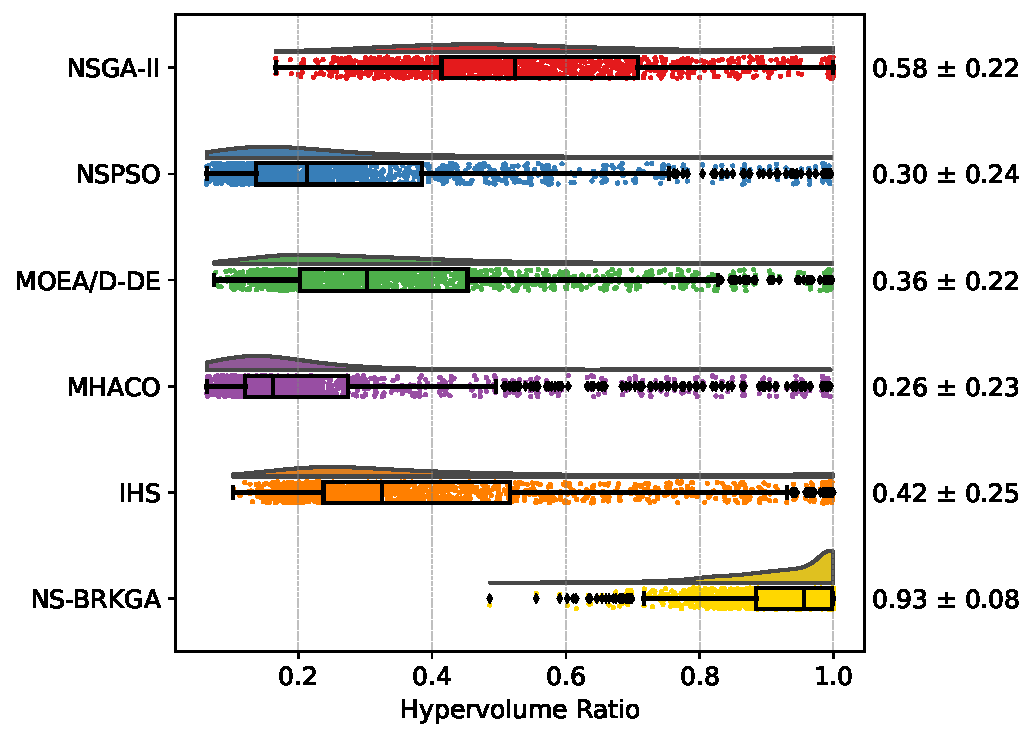
\includegraphics[width=0.48\textwidth]{figs/hypervolume.pdf}
\end{figure}

\vspace{-0.3em}
\begin{itemize}
\item \textsc{NS-BRKGA} attains the best mean ranks on \textbf{both} $\NIGDplus$ and $\HVR$.
\item Reported means: $\NIGDplus \approx 0.001$ and $\HVR \approx 0.93$ (\textsc{NSGA-II}: $0.009$ and $0.58$).
\end{itemize}

% Speaker note: Use this slide to make the main message unambiguous: “best overall, and with low variability”.
\end{frame}

%----------------------------------------------------------------------------------------
\begin{frame}
\frametitle{Scalability with problem size}

\begin{figure}
\centering
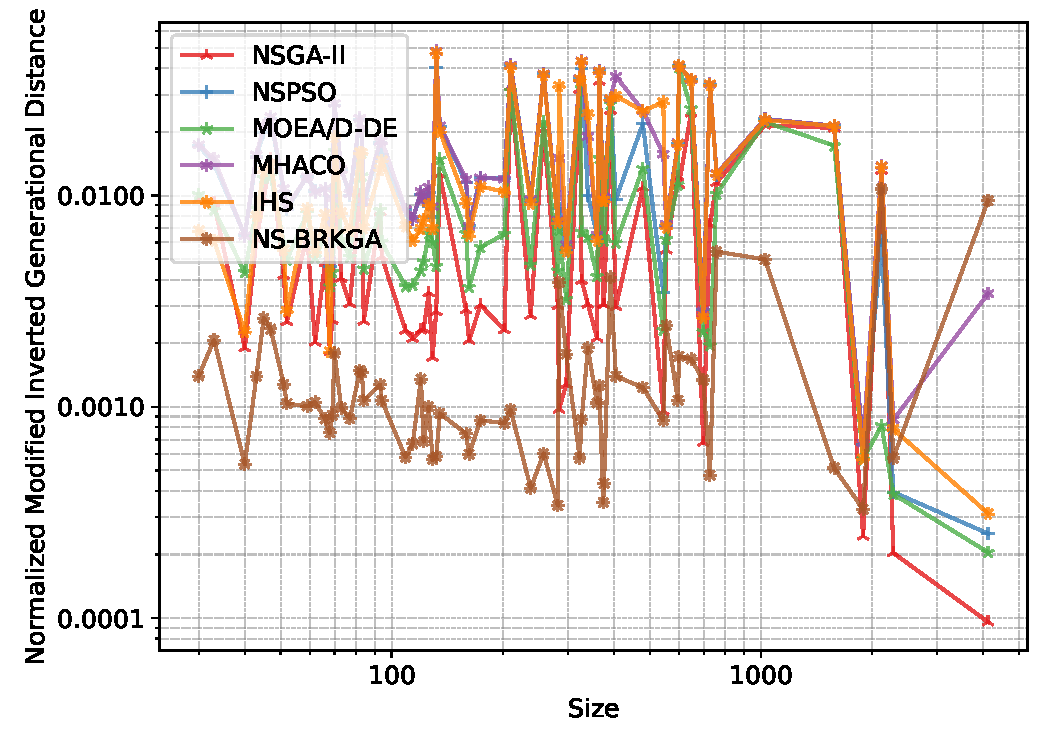
\includegraphics[width=0.48\textwidth]{figs/igd_plus_mean_per_size.pdf}
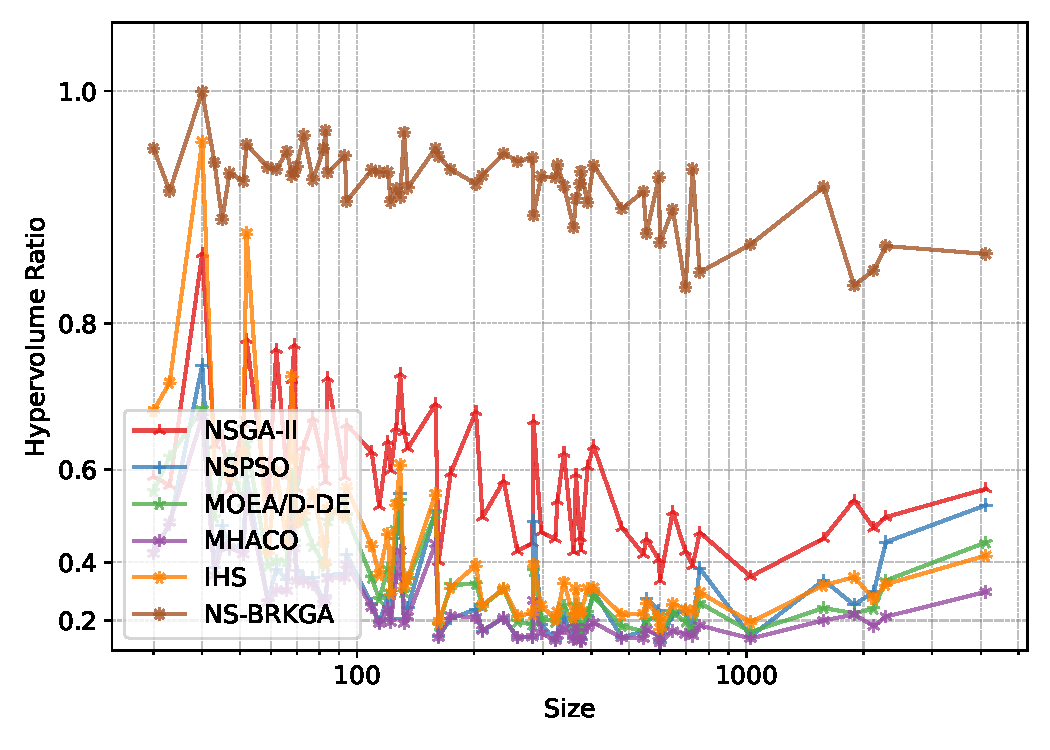
\includegraphics[width=0.48\textwidth]{figs/hypervolume_mean_per_size.pdf}
\end{figure}

\vspace{-0.3em}
\begin{itemize}
\item As $|V|$ grows, baseline methods degrade markedly, while \textsc{NS-BRKGA} remains stable.
\item On the largest instances ($|V| = 4125$), \textsc{NS-BRKGA} maintains mean $\HVR \approx 0.87 \pm 0.08$ (\textsc{NSGA-II} $\approx 0.6 \pm 0.1$).
\end{itemize}

% Speaker note: Interpret the curves: NS-BRKGA’s advantage widens at scale.
\end{frame}

%----------------------------------------------------------------------------------------
\begin{frame}
\frametitle{Robustness across instance types (constraint tightness)}

\begin{table}[!htbp]
% \caption{Mean $\NIGDplus$ ($\downarrow$) and $\HVR$ ($\uparrow$) by instance type.}
\label{table:robustness}
\centering
\resizebox{\textwidth}{!}{
\begin{tabular}{lcccccc}
\toprule
Algorithm          &                    \multicolumn{3}{c}{$\NIGDplus$ ($\downarrow$)}                    &                    \multicolumn{3}{c}{$\HVR$ ($\uparrow$)}                     \\
\cmidrule{2-7}
                   &        \texttt{full}       &       \texttt{orig}        &       \texttt{squz}        &      \texttt{full}       &      \texttt{orig}       &      \texttt{squz}       \\
\midrule
\textsc{NSGA-II}   &     $0.005 \pm 0.006$      &     $0.004 \pm 0.004$      &     $0.017 \pm 0.032$      &     $0.46 \pm 0.17$      &     $0.51 \pm 0.11$      &     $0.77 \pm 0.23$      \\
\textsc{NSPSO}     &     $0.011 \pm 0.007$      &     $0.011 \pm 0.006$      &     $0.029 \pm 0.037$      &     $0.22 \pm 0.14$      &     $0.20 \pm 0.11$      &     $0.49 \pm 0.30$      \\
\textsc{MOEA/D-DE} &     $0.007 \pm 0.005$      &     $0.006 \pm 0.004$      &     $0.017 \pm 0.030$      &     $0.27 \pm 0.12$      &     $0.30 \pm 0.13$      &     $0.53 \pm 0.27$      \\
\textsc{MHACO}     &     $0.011 \pm 0.007$      &     $0.011 \pm 0.007$      &     $0.033 \pm 0.039$      &     $0.15 \pm 0.07$      &     $0.17 \pm 0.09$      &     $0.47 \pm 0.30$      \\
\textsc{IHS}       &     $0.008 \pm 0.005$      &     $0.007 \pm 0.004$      &     $0.033 \pm 0.040$      &     $0.33 \pm 0.17$      &     $0.36 \pm 0.16$      &     $0.57 \pm 0.30$      \\
\textsc{NS-BRKGA}  & $\mathbf{0.001 \pm 0.001}$ & $\mathbf{0.001 \pm 0.001}$ & $\mathbf{0.002 \pm 0.007}$ & $\mathbf{0.90 \pm 0.09}$ & $\mathbf{0.91 \pm 0.08}$ & $\mathbf{0.97 \pm 0.05}$ \\
\bottomrule
\end{tabular}
}
\end{table}

\vspace{-0.2em}
\begin{itemize}
\item \textsc{NS-BRKGA} is competitive on \texttt{full}/\texttt{orig} and decisively best on \texttt{squz}.
\item On \texttt{squz}: mean $\HVR \approx 0.97$ and mean $\NIGDplus \approx 0.002$.
\end{itemize}

% Speaker note: Highlight the “small and fragmented feasible region” narrative: this supports why repair + feedback matters.
\end{frame}

%----------------------------------------------------------------------------------------
\begin{frame}
\frametitle{Runtime behavior: strong early convergence}

\begin{figure}
\centering
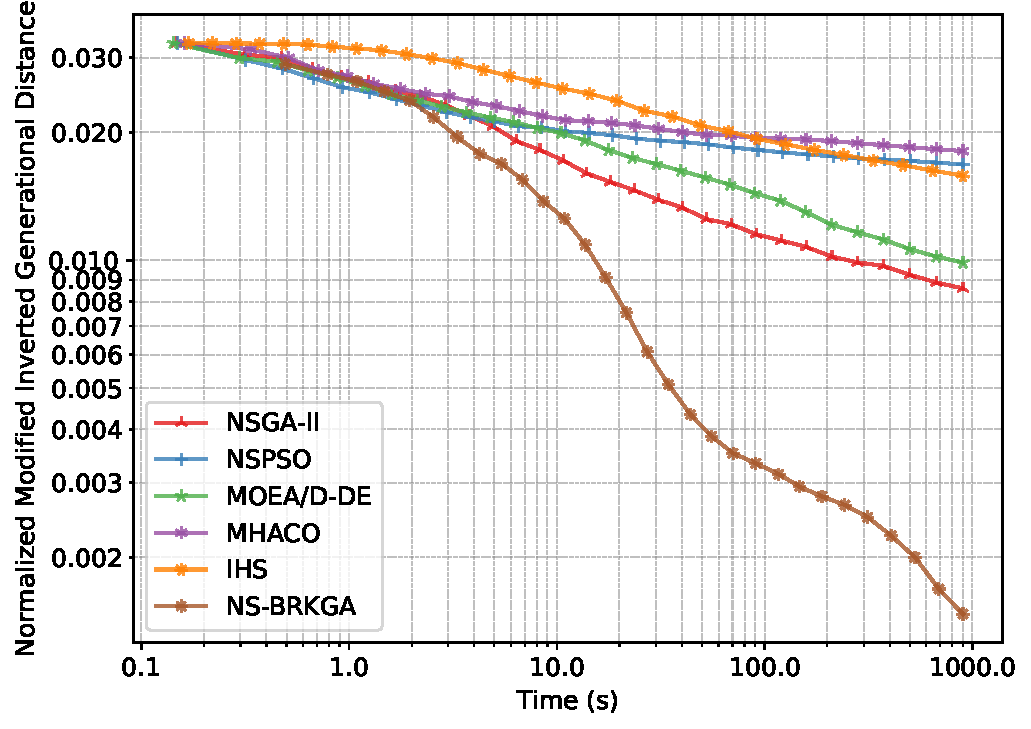
\includegraphics[width=0.48\textwidth]{figs/igd_plus_mean_snapshots.pdf}
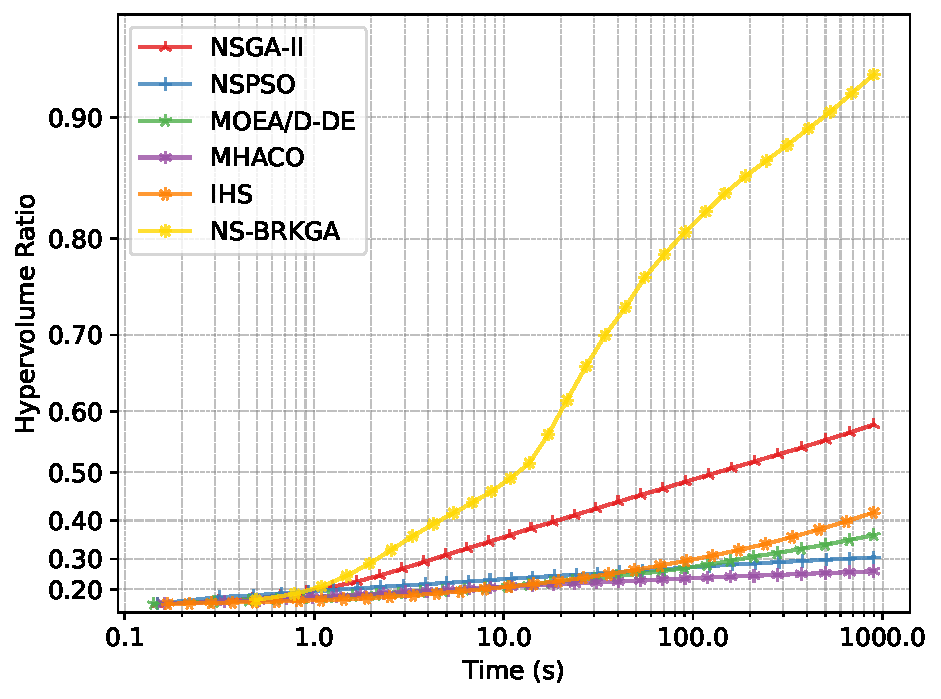
\includegraphics[width=0.48\textwidth]{figs/hypervolume_mean_snapshots.pdf}
\end{figure}

\vspace{-0.3em}
\begin{itemize}
\item \textsc{NS-BRKGA} reaches high-quality fronts \textbf{very early} (paper reports within $\sim 30$s: $\HVR \approx 0.7 \pm 0.2$).
\item Baselines often do not match this quality even after the full $15$-minute budget.
\end{itemize}

% Speaker note: This is a helpful slide for audiences who believe “memetic algorithms are slow”. Here, intensification pays off fast.
\end{frame}

%========================================================================================
\section{Key takeaways}

\begin{frame}[plain]
\begin{center}
{\Huge Key\\takeaways}
\end{center}
\end{frame}

%----------------------------------------------------------------------------------------
\begin{frame}
\frametitle{What to remember}

\begin{itemize}
\item The MOPCI is a large-scale \textbf{constrained} MOP requiring trade-offs among interference, deployment safety, and stability.

\item \textsc{NS-BRKGA}’s advantage comes from a \textbf{memetic decoder}:
\begin{itemize}
\item fast feasibility repair,
\item lexicographic local search reflecting operational priorities,
\item genotype feedback to inherit improvements.
\end{itemize}

\item On $291$ real-world instances, \textsc{NS-BRKGA} yields \textbf{better Pareto fronts} than five MOEA baselines under the same time budget, and scales to thousands of cells.
\end{itemize}

% Speaker note: Connect back to contributions slide. Keep it crisp.
\end{frame}

%========================================================================================
\section{Conclusions and future work}

\begin{frame}[plain]
\begin{center}
{\Huge Conclusions\\and future work}
\end{center}
\end{frame}

%----------------------------------------------------------------------------------------
\begin{frame}
\frametitle{Conclusions and future work}

\begin{itemize}
\item We introduced a memetic \textsc{NS-BRKGA} for the multi-objective PCI assignment problem, combining a problem-agnostic evolutionary engine with a problem-specific decoder.

\item The method provides a robust way to navigate trade-offs in LTE/5G network planning, showing strong performance, scalability, and robustness on highly constrained instances.

\item Future work mentioned in the paper:
\begin{itemize}
\item exact-solver comparisons on smaller instances (MIP formulation exists but is prohibitive at scale),
\item extensions to richer network models (e.g., heterogeneous multi-layer networks),
\item incorporation of additional operational/technological constraints when needed.
\end{itemize}
\end{itemize}

% Speaker note: End with one forward-looking sentence that connects to MIC community interests (hybridization, constraint handling, real-world benchmarking).
\end{frame}

%----------------------------------------------------------------------------------------
\begin{frame}
\frametitle{Thank you!}
\centering

\bigskip
Questions?

\bigskip
\small
\texttt{luis.mendes@ic.unicamp.br}

\medskip
{\scriptsize (Code and benchmark links are provided in the paper.)}
\end{frame}

%----------------------------------------------------------------------------------------

\end{document} 